\documentclass[aspectratio=169,11pt]{beamer}
\usepackage[T1]{fontenc}
\usepackage[utf8]{inputenc}
\usepackage{lmodern,amsmath,amssymb,graphicx}
\DeclareUnicodeCharacter{2013}{\ensuremath{-}}
\usetheme{default}
\usefonttheme{serif}
\setbeamercolor{normal text}{fg=black,bg=white}
\setbeamercolor{structure}{fg=black}
\setbeamercolor{frametitle}{fg=black}
\setbeamercolor{title}{fg=black}
\setbeamertemplate{navigation symbols}{}
\setbeamertemplate{footline}[frame number]
\setbeamertemplate{itemize items}[circle]
\setbeamersize{text margin left=8mm,text margin right=8mm}
\setlength{\parskip}{5pt}
\newcommand{\db}{\bar\partial}
\newcommand{\C}{\mathbb C}
\newcommand{\R}{\mathbb R}
\newcommand{\Z}{\mathbb Z}
\newcommand{\A}{\mathcal A}
\newcommand{\F}{\mathcal F}
\newcommand{\Lie}{\mathcal L}
\newcommand{\ee}{e_{n,m}}
\newcommand{\pbarz}{\partial_{\bar z}}
\newcommand{\src}[1]{\par\vfill{\scriptsize #1\par}}
\title{Lecture 13}
\subtitle{Local Dolbeault exactness and Hartogs extension}
\author{Daniel Gonz\'alez Casanova Azuela}
\date{}
\hypersetup{pdfauthor={Daniel Gonzalez Casanova Azuela},
 pdftitle={Lecture 13: Local Dolbeault exactness and Hartogs extension}}

\begin{document}
\begin{frame}
\titlepage
\end{frame}

\section{Dolbeault's theorem and sheaf cohomology}
\begin{frame}{Dolbeault's theorem: sheaves and sections}
Fix $p$ on a complex manifold $M$. For each open set $U\subset M$,
\[
 \Omega^p_M(U)=\{\text{holomorphic }p\text{-forms on }U\},\qquad
 \A^{p,q}_M(U)=\{\text{smooth }(p,q)\text{-forms on }U\}.
\]
A differential form is a \textbf{section} of a bundle of exterior powers
of the cotangent bundle. Assigning these sections to every open $U$,
with restriction maps, gives its \textbf{sheaf of sections}.

Taking \textbf{global sections} means evaluating the sheaf on $M$:
\[
 \Gamma(M,\A^{p,q}_M)=\A^{p,q}_M(M).
\]
Dolbeault's theorem identifies sheaf cohomology with the cohomology
of the global smooth-form complex:
\[
 \boxed{H^q(M,\Omega^p_M)\cong H^{p,q}_{\db}(M).}
\]
\end{frame}

\begin{frame}{Stalks and exactness}
The \textbf{stalk} $\F_x$ consists of germs $[s]_x$ of sections near $x$.
Two sections have the same germ if they agree on some smaller
neighbourhood of $x$. In particular,
\[
 [s]_x=0
 \quad\Longleftrightarrow\quad
 s|_V=0\ \text{for some neighbourhood }V\text{ of }x.
\]
A complex of sheaves is \textbf{exact at $\mathcal G$} precisely when
\[
 \F\xrightarrow{a}\mathcal G\xrightarrow{b}\mathcal H,
 \qquad
 \ker b_x=\operatorname{im}a_x\quad\text{for every }x.
\]
Thus a section of $\ker b$ must lift through $a$ \textbf{locally near
each point}. Different neighbourhoods may have different lifts.

A \textbf{lift} of $s$ on $V$ means a section $t\in\F(V)$ satisfying
$a(t)=s|_V$.
\end{frame}

\begin{frame}{Sheafification and global sections}
For a sheaf map $\varphi:\F\to\mathcal G$, the image presheaf
\[
 U\longmapsto\operatorname{im}\bigl(\F(U)\xrightarrow{\varphi_U}
 \mathcal G(U)\bigr)
\]
may fail the gluing axiom. Its \textbf{sheafification} is the
\textbf{image sheaf} $\operatorname{im}\varphi$.

A section $s\in\mathcal G(U)$ belongs to this image sheaf precisely
when some open cover $U=\bigcup_i U_i$ admits local lifts:
\[
 t_i\in\F(U_i),\qquad\varphi(t_i)=s|_{U_i}.
\]
The images $s|_{U_i}$ agree on overlaps, but the lifts $t_i$ need not glue.

Thus a \textbf{surjective sheaf map} guarantees local lifts.
The global-sections functor $\Gamma(M,-)$ asks for a lift on all of $M$,
which may not exist. This is why it can fail to be right exact.

\textbf{Sheafification includes sections with local lifts.
It does not guarantee a global lift.}
\end{frame}

\begin{frame}{The $\db$-Poincar\'e lemma on stalks}
Fix $x\in M$ and $q>0$. Take
$[\alpha]_x\in\ker(\db:\A^{p,q}_{M,x}\to\A^{p,q+1}_{M,x})$.
\begin{enumerate}
\item Choose a representative $\alpha$ on a neighbourhood $U$ of $x$.
The equation $[\db\alpha]_x=0$ lets us shrink to $V\subset U$ with
$\db\alpha|_V=0$.
\item The local $\db$-Poincar\'e lemma gives a smaller
$W\subset V$ and a $(p,q-1)$-form $\beta$ with
$\alpha|_W=\db\beta$.
\item Therefore $[\alpha]_x=\db[\beta]_x$.
The reverse inclusion follows from $\db^2=0$.
\end{enumerate}
In degree $0$, $\db\alpha=0$ means that the coefficients of the
$(p,0)$-form $\alpha$ are holomorphic. Hence the sheaf sequence
\[
 0\longrightarrow\Omega^p_M\longrightarrow\A^{p,0}_M
 \xrightarrow{\db}\A^{p,1}_M\xrightarrow{\db}\cdots
\]
is exact: it is a \textbf{resolution of $\Omega^p_M$}.
For $\dim_{\C}M>1$, this uses the several-variable local lemma.
\end{frame}

\begin{frame}{Global sections can lose exactness}
Applying $\Gamma(M,-)$ to the resolution gives the complex
\[
 \A^{p,0}_M(M)\xrightarrow{\db}\A^{p,1}_M(M)
 \xrightarrow{\db}\A^{p,2}_M(M)\longrightarrow\cdots.
\]
For $q>0$, its cohomology is, by definition,
\[
 H^{p,q}_{\db}(M)=
 \frac{\ker(\db:\A^{p,q}_M(M)\to\A^{p,q+1}_M(M))}
 {\operatorname{im}(\db:\A^{p,q-1}_M(M)\to\A^{p,q}_M(M))}.
\]
(Dolbeault cohomology can be nontrivial even coming from an exact
resolution.) Local primitives need not agree on overlaps, so they need not give
a global primitive. The global-sections functor is \textbf{left exact}:
it preserves kernels, but a surjective sheaf map need not be
surjective on global sections.

For example, on our elliptic curve, $d\bar z$ is locally $\db\bar z$
but has no global primitive. Thus $H^{0,1}_{\db}(E)=\C$,
although the sheaf sequence is exact.
\end{frame}

\begin{frame}{The other resolution: the definition of sheaf cohomology}
Work with sheaves of abelian groups.
An \textbf{injective sheaf} $\mathcal I$ has the extension property:
every map $\F'\to\mathcal I$ extends across an inclusion
$\F'\hookrightarrow\F$.

Every sheaf $\F$ admits an \textbf{injective resolution}, an exact
sequence whose terms $\mathcal I^r$ are injective:
\[
 0\longrightarrow\F\longrightarrow\mathcal I^0
 \xrightarrow{d^0}\mathcal I^1\xrightarrow{d^1}\cdots.
\]
Sheaf cohomology is defined by taking global sections first,
then cohomology:
\[
 H^q(M,\F):=R^q\Gamma(M,-)(\F)
 =H^q\bigl(\Gamma(M,\mathcal I^\bullet)\bigr).
\]
Here $R^q\Gamma$ denotes the $q$th right derived functor of $\Gamma$.
The result is independent of the chosen injective resolution,
up to canonical isomorphism.

For Dolbeault's theorem, take $\F=\Omega^p_M$.
\src{Voisin, Chapter 4, Lemma 4.26, Theorem 4.28 and Section 4.3.}
\end{frame}

\begin{frame}{Fine sheaves and acyclic resolutions}
A sheaf $\mathcal G$ is \textbf{acyclic for global sections} if
\[
 H^k(M,\mathcal G)=0\qquad(k>0).
\]
In Voisin's convention, a \textbf{fine sheaf} is a module sheaf over
a ring sheaf admitting locally finite partitions of unity
subordinate to open covers.

The sheaf $\A^{p,r}_M$ is a module over smooth functions.
Partitions of unity act by multiplication:
\[
 \alpha\longmapsto\chi_i\alpha,\qquad
 \sum_i\chi_i\alpha=\alpha.
\]
Thus each $\A^{p,r}_M$ is fine. Proposition 4.36 gives
\[
 H^k(M,\A^{p,r}_M)=0\qquad(k>0,\ \text{every }r).
\]
An \textbf{acyclic resolution} is an exact sheaf resolution whose
individual terms are acyclic. Local exactness comes from
$\db$-Poincar\'e, while acyclicity of the terms comes from fineness.
\src{Voisin, Definitions 4.31 and 4.35, Proposition 4.36.}
\end{frame}

\begin{frame}{Proposition 4.32 and Dolbeault's theorem}
\textbf{Proposition 4.32, for global sections.}
If $0\to\F\to\mathcal C^0\to\mathcal C^1\to\cdots$ is exact and
each $\mathcal C^r$ is acyclic, then
\[
 H^q(M,\F)\cong H^q\bigl(\Gamma(M,\mathcal C^\bullet)\bigr).
\]
For $\F=\Omega^p_M$, compare the Dolbeault and injective resolutions:
\begin{columns}[c,onlytextwidth]
\begin{column}{0.36\textwidth}
\fbox{\parbox[c]{\dimexpr\linewidth-2\fboxsep-2\fboxrule\relax}{
\centering\small
Cohomology of global sections\\
is, by definition, $H^{p,q}_{\db}(M)$.
}}
\end{column}
\begin{column}{0.61\textwidth}
\[
 0\longrightarrow\Omega^p_M\longrightarrow\A^{p,0}_M
 \xrightarrow{\db}\A^{p,1}_M\xrightarrow{\db}\cdots.
\]
\end{column}
\end{columns}

\medskip
\begin{columns}[c,onlytextwidth]
\begin{column}{0.36\textwidth}
\fbox{\parbox[c]{\dimexpr\linewidth-2\fboxsep-2\fboxrule\relax}{
\centering\small
Cohomology of global sections\\
$=H^q(M,\Omega^p_M)$.
}}
\end{column}
\begin{column}{0.61\textwidth}
\[
 0\longrightarrow\Omega^p_M\longrightarrow\mathcal I^0
 \longrightarrow\mathcal I^1\longrightarrow\cdots.
\]
\end{column}
\end{columns}

Both resolutions have acyclic terms, so Proposition 4.32 gives
\[
 \boxed{H^{p,q}_{\db}(M)\cong H^q(M,\Omega^p_M).}
\]
\src{Voisin, Proposition 4.32.}
\end{frame}

\begin{frame}{The homological algebra in degree one}
\textbf{This is how Proposition 4.32 works in the Dolbeault case.}

Let $\mathcal Z^1=\ker(\db:\A^{p,1}_M\to\A^{p,2}_M)$.
The local lemma gives a short exact sequence of sheaves:
\[
 0\longrightarrow\Omega^p_M\longrightarrow\A^{p,0}_M
 \xrightarrow{\db}\mathcal Z^1\longrightarrow0.
\]
Its long exact sequence in sheaf cohomology contains
\[
 \Gamma(M,\A^{p,0}_M)\xrightarrow{\db}\Gamma(M,\mathcal Z^1)
 \longrightarrow H^1(M,\Omega^p_M)
 \longrightarrow H^1(M,\A^{p,0}_M)=0.
\]
The final vanishing uses \textbf{fineness}. Exactness therefore gives
\[
 H^1(M,\Omega^p_M)\cong
 \frac{\Gamma(M,\mathcal Z^1)}
 {\db\,\Gamma(M,\A^{p,0}_M)}
 =H^{p,1}_{\db}(M).
\]
The numerator consists of global closed forms, and the denominator
of global exact forms. Repeating this argument with the successive
kernel sheaves proves the comparison in higher degrees.
\end{frame}

\begin{frame}{Pierre Dolbeault}
\centering
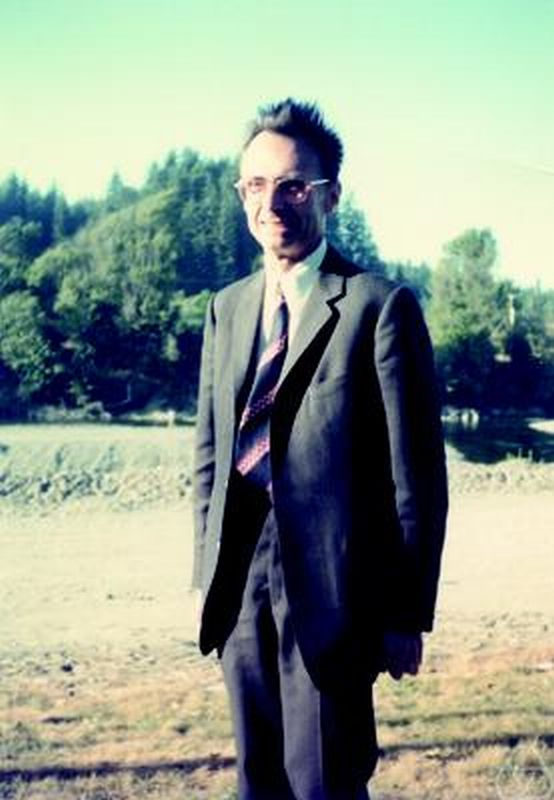
\includegraphics[width=0.9\textwidth,height=6cm,keepaspectratio]{Pierre_Dolbeault.jpg}
\end{frame}

\section{The local lemma in several variables}

\begin{frame}{The Poincar\'e--Dolbeault--Grothendieck lemma}
A \textbf{polydisk} is a product of disks
\[
 D=D_1\times\cdots\times D_n\subset\C^n.
\]
\textbf{Theorem.}
Let $\eta$ be a smooth $\db$-closed $(p,q)$-form on a neighbourhood
of $\overline D$, with $q>0$. Then there is a smooth $(p,q-1)$-form
$\beta$ on $D$ such that
\[
 \boxed{\eta|_D=\db\beta.}
\]
In particular, every $\db$-closed form of positive antiholomorphic
degree has a primitive \textbf{near each point}.

We will work inside a larger polydisk where $\eta$ is defined and
closed, and shrink finitely many times. This is enough for the
exactness on stalks used in the opening slides.
\src{Verbitsky, Lecture 13, pp.\ 5--10.}
\end{frame}

\begin{frame}{Proof outline: removing one direction at a time}
We want to write a closed form as $\eta=\db\beta$.
\begin{enumerate}
\item \textbf{Use the one-variable result.}
Solve $\partial_{\bar z_i}u=g$, treating the other coordinates as
parameters. The solution preserves holomorphic dependence on them.

\item \textbf{Subtract an exact correction.}
Choose $\beta_1$ so that $\eta-\db\beta_1$ has no $d\bar z_1$ term.
Closedness then forces its coefficients to be holomorphic in $z_1$.

\item \textbf{Repeat in the remaining variables.}
Each correction preserves the directions already removed.
After all $n$ directions, a form with $q>0$ must be zero.
Adding the corrections gives the required primitive.
\end{enumerate}
We first do this for $a\,d\bar z_1+b\,d\bar z_2$, then for general forms.
Misha's $R_i$ and $W_k$ will describe the same mechanism afterwards.
\end{frame}

\begin{frame}{Coordinates and the two operators}
Our conventions are
\[
 z=x+iy,\qquad dz=dx+i\,dy,\qquad d\bar z=dx-i\,dy,
 \qquad \partial_{\bar z}=\frac12(\partial_x+i\partial_y).
\]
For a smooth $(p,q)$-form $\alpha$, the operator
$\partial_{\bar z_i}$ differentiates its coefficients and keeps the
coordinate forms fixed. For example,
\[
 \partial_{\bar z_1}(f\,d\bar z_2)
 =(\partial_{\bar z_1}f)\,d\bar z_2.
\]
The Dolbeault operator also wedges with $d\bar z_i$:
\[
 \db_i\alpha=d\bar z_i\wedge\partial_{\bar z_i}\alpha,
 \qquad \db\alpha=\sum_{i=1}^n\db_i\alpha.
\]
Thus $\partial_{\bar z_i}$ preserves type, while $\db_i$ increases $q$ by one.
The wedge signs give
\[
 \db_i^2=0,\qquad \db_i\db_j+\db_j\db_i=0.
\]
\end{frame}


\begin{frame}{The one-variable ingredient from Lecture 12}
On $E=\C/(2\pi\Z+2\pi i\Z)$, write a smooth function as
\[
 g=\sum_{n,m}g_{n,m}e_{n,m},\qquad e_{n,m}=e^{inx+imy}.
\]
Since
\[
 \partial_{\bar z}e_{n,m}=\frac{in-m}{2}e_{n,m},
\]
we can divide every nonconstant mode by its eigenvalue:
\[
 Pg=\sum_{(n,m)\ne(0,0)}\frac{2g_{n,m}}{in-m}e_{n,m},
 \qquad \partial_{\bar z}Pg=g-g_{0,0}.
\]
Smooth Fourier coefficients decay faster than every power, so the
series and all its derivatives converge.

The remaining constant has the primitive $g_{0,0}\bar z$ on a disk.
This will give an operator $T$ with $\partial_{\bar z}Tg=g$.
\src{Lecture 12 recap; Verbitsky, Lecture 13, pp.\ 4, 6--7.}
\end{frame}

\begin{frame}{A linear solution operator on a disk}
Choose disks $\overline D\subset D^+$ inside a fundamental square of $E$.
We can arrange this by rescaling the coordinate.
Fix a \textbf{bump function} $\chi$ supported in $D^+$ and equal to $1$
near $\overline D$.

For $g\in C^\infty(D^+)$, extend $\widetilde g=\chi g$ by zero to $E$ and set
\[
 c=\frac1{(2\pi)^2}\int_E\widetilde g\,dx\,dy,\qquad
 Tg=(P\widetilde g)|_D+c\bar z.
\]
The Fourier formula gives $\partial_{\bar z}P\widetilde g=\widetilde g-c$.
Consequently,
\[
 \boxed{\partial_{\bar z}Tg=g\quad\hbox{on }D.}
\]
The operator $T$ is linear because the bump function is fixed.

\textbf{On the torus, $\bar z$ is not a global function.
On the disk it is available and removes the constant term.}
\src{Verbitsky, Lecture 13, pp.\ 4, 6--7.}
\end{frame}

\begin{frame}{Why the solution operator works with parameters}
Suppose $g=g(z,w)$ is smooth, where $w$ denotes the other coordinates.
Apply $T$ only in $z$, with the same bump function for every $w$.

Multiplication by $\chi$, Fourier coefficients, and the average
all operate only in $z$. Hence
\[
 \partial_{\bar w_j}(Tg)=T(\partial_{\bar w_j}g),
 \qquad
 \partial_{w_j}(Tg)=T(\partial_{w_j}g).
\]
These identities hold for all parameter derivatives. Smoothness follows
from rapid Fourier decay, uniformly on compact sets of parameters.

In particular,
\[
 \partial_{\bar w_j}g=0
 \quad\Longrightarrow\quad
 \partial_{\bar w_j}(Tg)=0.
\]
\textbf{Solving in one variable preserves holomorphic dependence
on the other variables.}
\end{frame}


\begin{frame}{Two variables: what are we trying to solve?}
Let
\[
 \alpha=a\,d\bar z_1+b\,d\bar z_2
\]
be a smooth $(0,1)$-form on a bidisk, with $\db\alpha=0$.
The coefficients $a,b$ may depend on both coordinates and their conjugates.

We want a function $u$ such that
\[
 \db u=(\partial_{\bar z_1}u)\,d\bar z_1
       +(\partial_{\bar z_2}u)\,d\bar z_2=\alpha.
\]
Equivalently, we want to solve both equations
\[
 \boxed{\partial_{\bar z_1}u=a,\qquad\partial_{\bar z_2}u=b.}
\]
The condition $\db\alpha=0$ makes these equations compatible.
We allow a smaller bidisk at each use of the one-variable operator.
\end{frame}

\begin{frame}{Closedness is the compatibility condition}
For $\alpha=a\,d\bar z_1+b\,d\bar z_2$, expand
\[
 \begin{aligned}
 \db\alpha
 &=\db a\wedge d\bar z_1+\db b\wedge d\bar z_2\\
 &=(\partial_{\bar z_2}a)\,d\bar z_2\wedge d\bar z_1
  +(\partial_{\bar z_1}b)\,d\bar z_1\wedge d\bar z_2\\
 &=\bigl(\partial_{\bar z_1}b-\partial_{\bar z_2}a\bigr)
       d\bar z_1\wedge d\bar z_2.
 \end{aligned}
\]
Here we used
\[
 d\bar z_i\wedge d\bar z_i=0,\qquad
 d\bar z_2\wedge d\bar z_1=-d\bar z_1\wedge d\bar z_2.
\]
The basis form $d\bar z_1\wedge d\bar z_2$ is nonzero. Hence
\[
 \boxed{\db\alpha=0\quad\Longleftrightarrow\quad
 \partial_{\bar z_1}b=\partial_{\bar z_2}a.}
\]
This is also necessary for a solution: the mixed derivatives of $u$ commute.
\end{frame}

\begin{frame}{First correction: removing the $d\bar z_1$ term}
Apply the one-variable operator in $z_1$, with $z_2$ as a parameter:
\[
 u_1=T_1a,\qquad \partial_{\bar z_1}u_1=a.
\]
Its full Dolbeault derivative is
\[
 \db u_1=a\,d\bar z_1+(\partial_{\bar z_2}u_1)\,d\bar z_2.
\]
Subtracting it gives
\[
 \boxed{\alpha-\db u_1=r\,d\bar z_2,\qquad
 r=b-\partial_{\bar z_2}u_1.}
\]
\textbf{The first coefficient is now correct.}
The remaining task is to find $u_2$ with
\[
 \partial_{\bar z_2}u_2=r,\qquad \partial_{\bar z_1}u_2=0.
\]
The second condition ensures that adding $u_2$ keeps the first equation solved.
\end{frame}

\begin{frame}{Why the remainder is holomorphic in $z_1$}
Recall $r=b-\partial_{\bar z_2}u_1$ and $\partial_{\bar z_1}u_1=a$.
Then
\[
 \begin{aligned}
 \partial_{\bar z_1}r
 &=\partial_{\bar z_1}b
   -\partial_{\bar z_1}\partial_{\bar z_2}u_1\\
 &=\partial_{\bar z_1}b
   -\partial_{\bar z_2}\partial_{\bar z_1}u_1\\
 &=\partial_{\bar z_1}b-\partial_{\bar z_2}a\\
 &=0.
 \end{aligned}
\]
The last equality is exactly the condition $\db\alpha=0$.

\textbf{The remainder has no $d\bar z_1$ term, and its coefficient is
holomorphic in $z_1$.}
It may still depend on $\bar z_2$.
\end{frame}

\begin{frame}{Second correction: keeping the first equation solved}
Solve in $z_2$:
\[
 u_2=T_2r,\qquad \partial_{\bar z_2}u_2=r.
\]
The parameter property of $T_2$ gives
\[
 \partial_{\bar z_1}u_2
 =T_2(\partial_{\bar z_1}r)=T_2(0)=0.
\]
Thus $\db u_2=r\,d\bar z_2$, and
\[
 \boxed{\alpha=\db u_1+r\,d\bar z_2=\db(u_1+u_2).}
\]
We solved the two equations successively. Closedness and the parameter
property ensured that the second correction preserved the first equation.
\end{frame}

\begin{frame}{General forms: the same first correction}
For a closed $(p,q)$-form $\eta$, collect all terms containing $d\bar z_i$:
\[
 \eta=d\bar z_i\wedge\beta+\delta.
\]
Neither $\beta$ nor $\delta$ contains $d\bar z_i$.
Moving $d\bar z_i$ to the front includes the appropriate wedge signs.

Apply $T_i$ to each coefficient of $\beta$ and set $v=T_i\beta$.
On a smaller polydisk,
\[
 \db v=d\bar z_i\wedge\beta
       +\sum_{j\ne i}d\bar z_j\wedge\partial_{\bar z_j}v.
\]
The sum has no $d\bar z_i$. Therefore
\[
 \boxed{\rho=\eta-\db v\quad\hbox{has no }d\bar z_i.}
\]
In the bidisk example, $\beta=a$ and $v=u_1=T_1a$.
The correction $v$ has type $(p,q-1)$.
\end{frame}

\begin{frame}{Closedness again controls the remainder}
The remainder $\rho=\eta-\db v$ is still closed:
\[
 \db\rho=\db\eta-\db^2v=0.
\]
Since $\rho$ contains no $d\bar z_i$, in the expression
\[
 0=\db\rho
  =d\bar z_i\wedge\partial_{\bar z_i}\rho
   +\sum_{j\ne i}d\bar z_j\wedge\partial_{\bar z_j}\rho
\]
only the first term contains $d\bar z_i$. Coordinate wedge monomials
are linearly independent, so that term vanishes separately.

Since $\partial_{\bar z_i}\rho$ also has no $d\bar z_i$, this gives
\[
 \boxed{\partial_{\bar z_i}\rho=0.}
\]
The coefficients of $\rho$ are holomorphic in $z_i$.
This is the general version of the calculation $\partial_{\bar z_1}r=0$.
\end{frame}

\begin{frame}{Why later corrections preserve earlier ones}
Suppose direction $j$ is already removed: the current form has no
$d\bar z_j$, and all its coefficients are holomorphic in $z_j$.

To remove a new direction $i\ne j$, write
$\eta=d\bar z_i\wedge\beta+\delta$ and take $v=T_i\beta$.
The form $\beta$ still has both properties in direction $j$, so
\[
 v\hbox{ has no }d\bar z_j,\qquad
 \partial_{\bar z_j}v=T_i(\partial_{\bar z_j}\beta)=0.
\]
Consequently $\db v$ also has no $d\bar z_j$. Moreover,
\[
 \partial_{\bar z_j}(\eta-\db v)
 =\partial_{\bar z_j}\eta-\db(\partial_{\bar z_j}v)=0.
\]
\textbf{The new remainder keeps both properties in every direction
already removed.}
This is why the one-variable operator had to work with parameters.
\end{frame}

\begin{frame}{Finishing the proof one coordinate at a time}
Choose nested polydisks inside the neighbourhood where $\eta$ is closed:
\[
 \overline{P_i}\subset P_{i-1}\quad(1\le i\le n),\qquad P_n=D.
\]
Start with $\eta_0=\eta|_{P_0}$. At step $i$, the preceding construction gives
\[
 \eta_i=\eta_{i-1}|_{P_i}-\db v_i.
\]
The form $\eta_i$ is closed and has no
$d\bar z_1,\ldots,d\bar z_i$. Its coefficients are holomorphic
in $z_1,\ldots,z_i$.

After $n$ steps, $\eta_n$ has no antiholomorphic differentials.
Since its antiholomorphic degree is $q>0$, we have $\eta_n=0$.
Adding the corrections, restricted to $D$, gives
\[
 \boxed{\eta|_D=\db(v_1|_D+\cdots+v_n|_D).}
\]
This proves the lemma. Next we express these corrections in Misha's notation.
\end{frame}

\begin{frame}{Misha's notation: a removed direction is $R_i$}
We have used two conditions together. A form belongs to $R_i(P)$ when
\begin{itemize}
\item no coordinate wedge monomial contains $d\bar z_i$;
\item every coefficient is holomorphic in $z_i$:
$\partial_{\bar z_i}\alpha=0$.
\end{itemize}
In our bidisk example,
\[
 \alpha-\db u_1=r\,d\bar z_2\in R_1,
 \qquad\partial_{\bar z_1}r=0.
\]
In the proof just completed, each successive remainder lies in
\[
 R_1,\qquad R_1\cap R_2,\qquad\ldots,\qquad R_1\cap\cdots\cap R_n.
\]
Misha combines the corrections in all coordinates symmetrically.
His spaces $W_k$ will keep track of sums of forms with $k$ directions removed.
\src{Verbitsky, Lecture 13, pp.\ 8--10.}
\end{frame}

\begin{frame}{Misha's correction operator $\gamma_i$}
Contraction $\kappa_i=\iota_{\partial_{\bar z_i}}$ removes $d\bar z_i$:
\[
 \eta=d\bar z_i\wedge\beta+\delta
 \quad\Longrightarrow\quad\kappa_i\eta=\beta,
\]
where $\beta,\delta$ have no $d\bar z_i$.
Thus our correction $v=T_i\beta$ is the operator
\[
 \gamma_i=T_i\kappa_i:
 \A^{p,q}(P)\longrightarrow\A^{p,q-1}(P'),
 \qquad\gamma_i\eta=T_i\beta.
\]
Here $\overline{P'}\subset P$, as in the preceding proof.
Define the degree-preserving operator
\[
 K_i=\db_i\gamma_i+\gamma_i\db_i.
\]
We next prove $\eta-K_i\eta\in R_i(P')$.
For closed forms, $K_i\eta$ will equal the exact correction $\db\gamma_i\eta$.
\end{frame}

\begin{frame}{The operator $K_i$ removes direction $i$}
Write $\eta=d\bar z_i\wedge\beta+\delta$ as before.
Since $\partial_{\bar z_i}T_i=\operatorname{Id}$ on the smaller disk,
\[
 \begin{aligned}
 \gamma_i\eta&=T_i\beta,\\
 \db_i\gamma_i\eta&=d\bar z_i\wedge\beta,\\
 \gamma_i\db_i\eta&=T_i\partial_{\bar z_i}\delta.
 \end{aligned}
\]
Therefore
\[
 \eta-K_i\eta=\delta-T_i\partial_{\bar z_i}\delta.
\]
This has no $d\bar z_i$, and its $\partial_{\bar z_i}$ derivative is zero.
Thus $\eta-K_i\eta\in R_i(P')$.

If $\eta\in R_i(P)$ already, then $\beta=0$ and
$\partial_{\bar z_i}\delta=0$, so $K_i\eta=0$.

For $j\ne i$, both $\gamma_i$ and $\db_i$ preserve the two $R_j$
conditions. Hence $K_i$ also preserves every previously removed direction.
\end{frame}

\begin{frame}{Why $K_i\eta$ is exact when $\eta$ is closed}
For $i\ne j$, the operator $T_i$ commutes with $\partial_{\bar z_j}$.
The wedge sign in contraction gives
\[
 \kappa_i(d\bar z_j\wedge\alpha)
 =-d\bar z_j\wedge\kappa_i\alpha,
 \qquad\db_j\gamma_i+\gamma_i\db_j=0.
\]
Hence all the mixed terms cancel:
\[
 \db\gamma_i+\gamma_i\db
 =\db_i\gamma_i+\gamma_i\db_i=K_i.
\]
For a closed form, this becomes $K_i\eta=\db\gamma_i\eta$,
which is exactly the correction used in the coordinate-by-coordinate proof.

Adding over $i$, set
\[
 \gamma=\sum_{i=1}^n\gamma_i,\qquad
 K=\sum_{i=1}^n K_i=\db\gamma+\gamma\db.
\]
For closed $\eta$, we also have $K\eta=\db\gamma\eta$.
\end{frame}

\begin{frame}{Misha's $W_k$: sums with $k$ directions removed}
When $n=2$, Misha groups together the two possible first corrections:
\[
 W_1=R_1+R_2,\qquad W_2=R_1\cap R_2.
\]
Thus $\rho\in W_1$ means $\rho=\rho_1+\rho_2$, with
$\rho_1\in R_1$ and $\rho_2\in R_2$.
The removed direction can differ between the summands.

In general, for fixed type $(p,q)$, set
\[
 W_0=\A^{p,q},\qquad
 W_k=\sum_{i_1<\cdots<i_k}R_{i_1}\cap\cdots\cap R_{i_k}.
\]
This is a \textbf{filtration}, meaning a nested sequence of spaces:
\[
 W_0\supset W_1\supset\cdots\supset W_n.
\]
In $W_n=R_1\cap\cdots\cap R_n$, all directions are removed.
Therefore $W_n=0$ when $q>0$.
\src{Verbitsky, Lecture 13, pp.\ 9--10.}
\end{frame}

\begin{frame}{Why Misha divides the correction by $n-k$}
Suppose $\alpha\in R_{i_1}\cap\cdots\cap R_{i_k}$.
There are $n-k$ directions still to remove.
\begin{itemize}
\item For an already removed direction, $K_i\alpha=0$.
\item For each remaining direction, $\alpha-K_i\alpha$ has that direction
removed as well, and keeps the previous $k$ conditions.
\end{itemize}
Adding these $n-k$ remainders gives
\[
 \sum_{i\notin\{i_1,\ldots,i_k\}}(\alpha-K_i\alpha)
 =(n-k)\alpha-K\alpha\in W_{k+1}.
\]
By linearity, this holds for every $\alpha\in W_k$.
If $\alpha$ is closed, then $K\alpha=\db\gamma\alpha$, so
\[
 \boxed{\alpha-\db\!\left(\frac{\gamma\alpha}{n-k}\right)
 \in W_{k+1}\qquad(k<n).}
\]
The division averages the corrections over the $n-k$ remaining directions.
\end{frame}

\begin{frame}{Misha's proof: successive exact corrections}
Use nested polydisks $\overline{P_{k+1}}\subset P_k$, with $P_n=D$,
and start with the closed form $\eta_0=\eta|_{P_0}$.

At stage $k$, suppose $\eta_k\in W_k$. On the next smaller polydisk, set
\[
 \beta_k=\frac{\gamma^{(k)}\eta_k}{n-k},\qquad
 \eta_{k+1}=\eta_k|_{P_{k+1}}-\db\beta_k.
\]
The superscript records the operator for $P_k$ and $P_{k+1}$.
The previous slide gives $\eta_{k+1}\in W_{k+1}$, and
$\db\eta_{k+1}=0$ because $\db^2=0$.

After $n$ stages, $\eta_n\in W_n=0$. Hence
\[
 \boxed{\eta|_D=\db\!\left(\sum_{k=0}^{n-1}\beta_k|_D\right).}
\]
This has the same structure as $\alpha=\db(u_1+u_2)$ in our example:
each exact correction simplifies the remainder until it vanishes.
\src{Verbitsky, Lecture 13, pp.\ 9--10.}
\end{frame}


\begin{frame}{The local input for Dolbeault's theorem is now proved}
Given a $\db$-closed form near a point of a complex manifold,
choose a coordinate chart and a polydisk whose closure lies in that chart.
The theorem supplies a primitive on this polydisk.

Thus, in positive degrees, the complex of sheaves
\[
 0\longrightarrow\Omega^p_M\longrightarrow\A^{p,0}_M
 \xrightarrow{\db}\A^{p,1}_M\xrightarrow{\db}\cdots
\]
is exact on every stalk.

The sheaves $\A^{p,q}_M$ are fine, hence acyclic for global sections.
The homological algebra from the opening now applies:
\[
 \boxed{H^q(M,\Omega^p_M)\cong H^{p,q}_{\db}(M).}
\]
Dolbeault's theorem holds for noncompact complex manifolds as well.
\end{frame}

\begin{frame}{Why the stronger open-polydisk statement is separate}
The proof used a larger domain where the form is smooth and closed.
This is sufficient for \textbf{local exactness}: around each point
we may choose a smaller polydisk with closure inside the given domain.

The stronger open-polydisk theorem assumes only
$\eta\in\A^{p,q}(D)$ and $\db\eta=0$, with $q>0$, and gives
\[
 \eta=\db\beta\quad\hbox{on all of }D,
\]
without any extension assumption at the boundary.
It implies the global vanishing
\[
 H^{p,q}_{\db}(D)=0\qquad(q>0).
\]
That stronger theorem is unnecessary for the fine-resolution proof
of Dolbeault's theorem. The distinction is \textbf{local primitives}
versus \textbf{one primitive on the whole original domain}.
\src{Huybrechts, Propositions 1.3.7--1.3.8 and Corollary 1.3.9.}
\end{frame}

\section{Hartogs extension}

\begin{frame}{Hartogs extension}
\textbf{Theorem.}
Let $n\ge2$, and let $K\subset\C^n$ be compact with
$\C^n\setminus K$ connected. Every holomorphic function
\[
 f:\C^n\setminus K\longrightarrow\C
\]
has a unique holomorphic extension to $\C^n$.

In particular, an isolated singularity is removable in dimension
at least two. In one variable, $f(z)=1/z$ on $\C\setminus\{0\}$
shows that this conclusion fails.

\textbf{Misha's proof strategy.}
Construct a smooth function $\widetilde f$ that equals $f$ outside
a compact set. Then find a compactly supported function $\psi$ with
\[
 \db\psi=\db\widetilde f.
\]
The difference $F=\widetilde f-\psi$ will be holomorphic.
\src{Verbitsky, Lecture 13, p.\ 11; connectedness is needed for agreement everywhere.}
\end{frame}

\begin{frame}{A smooth extension and its error}
Choose $R$ with $K\subset B_R$, and a smooth bump function $\chi$
equal to $1$ near $K$ and supported in $B_R$.
Define
\[
 \widetilde f=(1-\chi)f\quad\hbox{on }\C^n\setminus K,
\]
and set $\widetilde f=0$ near $K$.
The definitions agree because $1-\chi=0$ on a neighbourhood of $K$.

Thus $\widetilde f$ is smooth on $\C^n$ and equals $f$ outside $B_R$.
Its failure to be holomorphic is the form
\[
 \alpha=\db\widetilde f=-f\,\db\chi.
\]
This is a smooth $(0,1)$-form with
\[
 \db\alpha=0,\qquad \operatorname{supp}\alpha\subset\overline{B_R}.
\]
The \textbf{support} is the closure of the set where the form is nonzero.
\end{frame}

\begin{frame}{Putting the error on projective space}
The standard affine chart identifies
\[
 \C^n\longrightarrow\mathbb P^n,\qquad
 (z_1,\ldots,z_n)\longmapsto[1:z_1:\cdots:z_n].
\]
Its complement is the \textbf{hyperplane at infinity}
\[
 H_\infty=\{[Z_0:\cdots:Z_n]:Z_0=0\}\cong\mathbb P^{n-1}.
\]
Since $\alpha$ has compact support in $\C^n$, it vanishes on a
neighbourhood of $H_\infty$. Extending it by zero therefore gives
a smooth closed $(0,1)$-form on all of $\mathbb P^n$.

We want to use
\[
 H^{0,1}_{\db}(\mathbb P^n)=0
 \quad\Longrightarrow\quad
 \alpha=\db\varphi,\qquad\varphi\in C^\infty(\mathbb P^n).
\]
The next slide explains this vanishing.
\end{frame}

\begin{frame}{Why $H^{0,1}_{\db}(\mathbb P^n)=0$}
We use two facts:
\begin{itemize}
\item $\mathbb P^n$ is compact K\"ahler with its Fubini--Study metric.
\item $H^1_{\mathrm{dR}}(\mathbb P^n,\C)=0$.
The standard cell decomposition has one cell in each real dimension
$0,2,\ldots,2n$, and none in odd dimensions.
\end{itemize}
The K\"ahler Hodge theorem gives
\[
 H^1_{\mathrm{dR}}(\mathbb P^n,\C)
 \cong H^{1,0}_{\db}(\mathbb P^n)
 \oplus H^{0,1}_{\db}(\mathbb P^n).
\]
Since the left side is zero, both summands vanish. In particular,
\[
 \boxed{H^{0,1}_{\db}(\mathbb P^n)=0.}
\]
The passage from de Rham cohomology to Dolbeault cohomology here
uses \textbf{K\"ahlerness}.
\src{HP: Hodge theorem and Fubini--Study metric; Verbitsky, Lecture 13, p.\ 11.}
\end{frame}

\begin{frame}{A bounded solution of the error equation}
The vanishing just proved yields a smooth function
\[
 \varphi\in C^\infty(\mathbb P^n),\qquad \db\varphi=\alpha.
\]
Because $\mathbb P^n$ is compact, $\varphi$ is bounded.
On $\C^n\setminus\overline{B_R}$ we have $\alpha=0$, hence $\varphi$
is holomorphic there.

Moreover, $\varphi$ is holomorphic near $H_\infty$.
Its restriction to the compact connected manifold
$H_\infty\cong\mathbb P^{n-1}$ is therefore a constant $c$.

Here we use the maximum principle: a holomorphic function on a compact
connected complex manifold is constant.

We will show that
\[
 \varphi=c\quad\hbox{outside }\overline{B_R}.
\]
Then subtracting $c$ gives the compactly supported correction we need.
\end{frame}

\begin{frame}{Complex lines outside the ball}
Fix $z\in\C^n$ with $\lVert z\rVert>R$.
Since $n\ge2$, choose a unit vector $v$ Hermitian-orthogonal to $z$.
The affine complex line
\[
 L_z=\{z+t v:t\in\C\}
\]
misses $\overline{B_R}$, because
\[
 \lVert z+t v\rVert^2=\lVert z\rVert^2+|t|^2>R^2.
\]
The restriction $t\mapsto\varphi(z+t v)$ is entire and bounded.
By \textbf{Liouville's theorem}, it is constant.

As $t\to\infty$, the point $[1:z+t v]$ tends to $[0:v]\in H_\infty$,
where $\varphi=c$. Thus
\[
 \boxed{\varphi(z)=c\quad\hbox{for every }\lVert z\rVert>R.}
\]
This is the step that uses the extra complex direction.
\end{frame}

\begin{frame}{Finishing Hartogs extension}
Set
\[
 \psi=\varphi|_{\C^n}-c.
\]
Then $\psi$ has compact support and $\db\psi=\alpha$.
Therefore
\[
 F=\widetilde f-\psi,\qquad
 \db F=\alpha-\alpha=0,
\]
so $F$ is holomorphic on all of $\C^n$.

Outside $\overline{B_R}$, both $\widetilde f=f$ and $\psi=0$.
Thus $F=f$ on a nonempty open subset of $\C^n\setminus K$.
Since this complement is connected, the \textbf{identity theorem} gives
\[
 F|_{\C^n\setminus K}=f.
\]
The identity theorem also gives uniqueness.\hfill$\square$

Connectedness is used to recover agreement on the
\emph{whole} original domain, after the construction outside a larger ball.
\end{frame}

\begin{frame}{References}
\begin{itemize}
\item Misha Verbitsky, \emph{Hodge theory}, IMPA 2025,
Lecture 13: Poincar\'e--Dolbeault--Grothendieck lemma.
The homotopy construction and the Hartogs proof follow these slides.
\[
 \text{\href{http://verbit.ru/IMPA/Kahler-2025/slides-Kahler-2025-13.pdf}
 {verbit.ru/IMPA/Kahler-2025/slides-Kahler-2025-13.pdf}}
\]
\item Heap Project: complex geometry, complex analysis, and Hodge theory.
Notation for $\partial_{\bar z}$, $\db$, smooth forms and sheaves,
the identity theorem, and the K\"ahler Hodge theorem.

\item Claire Voisin, \emph{Hodge Theory and Complex Algebraic Geometry I},
Chapter 4: acyclic resolutions and fine sheaves.

\item Daniel Huybrechts, \emph{Complex Geometry: An Introduction},
Propositions 1.3.7--1.3.8 and Corollary 1.3.9.
\end{itemize}
\end{frame}

\end{document}
